\part{Matlab programming II}
\section{Coding style}
\subsection*{Introduction}
\begin{frame}[label=contents_prog2]
  \frametitle{Today's outline}
  \mode<beamer>{
    \only<1>{\tableofcontents}
  }
  \only<2>{\tableofcontents[currentsection]}
\end{frame}

\subsection*{Program design}
\begin{frame}[label=workrightfast]
  \frametitle{Make a habit of the following adage}
  \begin{center}
    
\includegraphics[width=0.8\textwidth]{workrightfast.pdf}
  \end{center}
\end{frame}

\begin{frame}[label=work-explain]
  \frametitle{Make it work}
  Use the building blocks of previous lecture to create an algorithm:
  \begin{enumerate}
    \colorize<1> \item \emph{Problem analysis}\\ Contextual understanding of the nature of the problem to be solved
    \colorize<2> \item \emph{Problem statement}\\ Develop a detailed statement of the mathematical problem to be solved with the program
    \colorize<3> \item \emph{Processing scheme}\\ Define the inputs and outputs of the program
    \colorize<4> \item \emph{Algorithm}\\ A step-by-step procedure of all actions to be taken by the program (\emph{pseudo-code})
    \colorize<5> \item \emph{Program the algorithm}\\ Convert the algorithm into a computer language, and debug until it runs
    \colorize<6> \item \emph{Evaluation}\\ Test all of the options and conduct a validation study
  \end{enumerate}
  \vskip1em
  Now it's time to make it right!
\end{frame}

% \subsection*{Program design and coding style}
% \begin{frame}
%   \frametitle{It's a bit disturbing but...}
%   \begin{center}
%     {\LARGE Your code will not be understood by anyone\\}
%   \pause
%   \vskip1em
%   That includes future-you
%   \vskip2em
%   \end{center}
% \end{frame}

\subsection*{Example code}
\begin{frame}[fragile]
 \frametitle{Interpret the following code}
 \begin{lstlisting}
s=checksc();
if(s==true)
a=cb();
b=cfrsp();
if(a<5)
if(b>5)
a=gtbs();
end
if(a>b)
ubx();
end
end
else
brn();
gtbs();
end
 \end{lstlisting}
\end{frame}

\begin{frame}[plain]

\includegraphics[keepaspectratio=true,width=\textwidth]{wat-2.jpg}
\end{frame}

\begin{frame}[fragile]
 \frametitle{Let's change that a bit... Indentation}
 \pause
 Shown here with 2 spaces of indentation, Matlab uses 4 by default!
 \begin{columns}[T]
    \column{0.4\textwidth}
     \begin{lstlisting}
s=checksc();
if(s==true)
a=cb();
b=cfrsp();
if(a<5)
if(b>5)
a=gtbs();
end
if(a>b)
ubx();
end
end
else
brn();
gtbs();
end
 \end{lstlisting}
    \column{0.6\textwidth}
     \begin{lstlisting}
s = checksc();
if (s == true)
  a = cb();
  b = cfrsp();
  if (a < 5)
    if (b > 5)
      a = gtbs();
    end
    if (a > b)
      ubx();
    end
  end
else
  brn();
  gtbs();
end
 \end{lstlisting}
 \end{columns}
\end{frame}

\begin{frame}[fragile]
 \frametitle{Readable variables and function names}
 \begin{columns}[T]
    \column{0.4\textwidth}
\begin{lstlisting}
s = checksc();
if (s == true)
  a = cb();
  b = cfrsp();
  if (a < 5)
    if (b > 5)
      a = gtbs();
    end
    if (a > b)
      ubx();
    end
  end
else
    brn();
    gtbs();
end
 \end{lstlisting}
    \column{0.6\textwidth}
     \begin{lstlisting}
IAmFree = checkSchedule();
if (IAmFree == true)
  books = countBooks();
  shelfSize = countFreeSpaceShelf();
  if (books < 5)
    if (shelfSize > 5)
      books = goToBookStore();
    end
    if (books > shelfSize)
      useBox();
    end
  end
else
  burnBooks();
  goToBookStore();
end
 \end{lstlisting}
 \end{columns}
%  \pause
%  \begin{itemize}
%   \item This style uses lowerCamelCase naming style. This is a personal preference.
%   \item Function names start with a verb; it \emph{does} something.
%  \end{itemize}
\end{frame}

\begin{frame}[fragile]
 \frametitle{Get rid of magic numbers in the code}
 \begin{columns}[T]
    \column{0.5\textwidth}
     \begin{lstlisting}[basicstyle=\scriptsize\ttfamily]
IAmFree = checkSchedule();
if (IAmFree == true)
  books = countBooks();
  shelfSize = countFreeSpaceShelf();
  if (books < 5)
    if (shelfSize > 5)
      books = goToBookStore();
    end
    if (books > shelfSize)
      useBox();
    end
  end
else
  burnBooks();
  goToBookStore();
end
 \end{lstlisting}
    \column{0.5\textwidth}
     \begin{lstlisting}[basicstyle=\scriptsize\ttfamily,emph={minBooksNeeded,maxShelfSize},emphstyle=\color{red}]
maxShelfSize = 5;
minBooksNeeded = 5;

IAmFree = checkSchedule();
if (IAmFree == true)
  books = countBooks();
  shelfSize = countFreeSpaceShelf();
  if (books < maxShelfSize)
    if (shelfSize > minBooksNeeded)
      books = goToBookStore();
    end
    if (books > shelfSize)
      useBox();
    end
  end
else
  burnBooks();
  goToBookStore();
end
 \end{lstlisting}
 \end{columns}
\end{frame}

\begin{frame}[fragile]
 \frametitle{That's more like it!}
 \begin{columns}[T]
    \column{0.3\textwidth}
     \begin{lstlisting}
s=checksc();
if(s==true)
a=cb();
b=cfrsp();
if(a<5)
if(b>5)
a=gtbs();
end
if(a>b)
ubx();
end
end
else
brn();
gtbs();
end
 \end{lstlisting}
    \column{0.7\textwidth}
     \begin{lstlisting}
maxShelfSize = 5;
minBooksNeeded = 5;

IAmFree = checkSchedule();
if (IAmFree == true)
  books = countBooks();
  shelfSize = countFreeSpaceShelf();
  if (books < maxShelfSize)
    if (shelfSize > minBooksNeeded)
      books = goToBookStore();
    end
    if (books > shelfSize)
      useBox();
    end
  end
else
  burnBooks();
  goToBookStore();
end
 \end{lstlisting}
 \end{columns}
\end{frame}

\subsection*{Aspects of a good program}
\begin{frame}
  \frametitle{Writing readable code}
  Good code reads like a book.\vskip2em \pause
  \begin{itemize}
    \item When it doesn't, make sure to use comments. In Matlab, everything following \lstinline$ \% is a comment$
    \item Prevent ``smart constructions'' in the code
    \item Re-use working code (i.e. create functions for well-defined tasks).
    \item Documentation is also useful, but hard to maintain.
    \item Matlab comes with a function that generates reports from comments
  \end{itemize}
\end{frame}

\begin{frame}[fragile]
 \frametitle{How not to comment}
 \begin{itemize}[<+->]
  \item Useless:
  \begin{lstlisting}
% Start program 
  \end{lstlisting}
  \item Obvious:
  \begin{lstlisting}
if (a > 5)   % Check if a is greater than 5
    ... 
end\end{lstlisting}
  \item Too much about the life:
  \begin{lstlisting}[basicstyle=\tiny\ttfamily]
% Well... I do not know how to explain what is going on
% in the snippet below. I tried to code in the night 
% with some booze and it worked then, but now I have a 
% strong hangover and some parameters still need to be
% worked out...
  \end{lstlisting}

  \item ...
  \begin{lstlisting}[basicstyle=\tiny\ttfamily]
% You may think that this function is obsolete, and doesn't seem to
% do anything. And you would be correct. But when we remove this 
% function for some reason the whole program crashes and we can't 
% figure out why, so here it will stay.
  \end{lstlisting}
 \end{itemize}
\end{frame}

\begin{frame}[fragile]
 \frametitle{Adding comments to our program}
 \centering\tikz{\node[emphblock, text width=0.7\textwidth]{Use comments to document design and purpose (functionality), not mechanics (implementation).};}
 \begin{lstlisting}
IAmFree = checkSchedule();
if (IAmFree == true)
% Count books and amount of free space on a shelf. 
% If minimum number of books I need is less than a 
% shelf capacity, go shopping and buy additional 
% literature. If the amount of books after the 
% shopping is too big, use boxes to store them.
  books = countBooks();
  shelfSize = countFreeSpaceShelf();
  
  ...

else
  burnBooks();
  goToBookStore();
end
 \end{lstlisting}
\end{frame}

% \begin{frame}
%   \frametitle{If anything sticks today, let it be this}
%   \begin{center}
%     {\LARGE Your code will not be understood by anyone\\}
%   \pause
%   \vskip1em
%   That includes future-you
%   \vskip2em
%   \end{center}
%   \pause
%   \tikz{\node[emphblock, text width=\textwidth]{Use comments and code to document design and purpose (functionality), not mechanics (implementation).};}
%   \vskip1em\pause
%   \tikz{\node[emphblock, text width=\textwidth]{Use consistent and sensible naming of functions and variables.};}
% \end{frame}

\begin{frame}
  \frametitle{What else makes a good program?}
  \begin{columns}[T]
        \column{0.5\textwidth}
        \begin{itemize}
            \item Portability (guaranteed in Matlab)
            \item Readability
            \item Efficiency 
            \item Structural
            \item Flexibility
            \item Generality
            \item Documentation
        \end{itemize}
        \column{0.5\textwidth}
Funny thing is: This list does not mention that the program should be actually working for its intended purposes!
    \end{columns}
\end{frame}

\begin{frame}[fragile]
  \frametitle{Portability}
  It should work on your neighbors laptop. Well, that is guaranteed anyway. There is a little caveat though, what if your neighbor is stupid and has a polluted workspace?
  \vspace*{2em}
  \begin{lstlisting}
   % trust no one! nuke all evidence! no witnesses!
   clear all   % destroy all variables
   close all   % close all figures
  \end{lstlisting}
  \vspace*{2em}
  Solution: clear all variables before your program starts
\end{frame}

\begin{frame}[fragile]
  \frametitle{Readability}
  Don’t use meaningless variable or function names. Rule of thumb: use verbs for functions and nouns for variables.
  \vspace*{2em}
  \begin{lstlisting}
   % stupid names
   x = 5;
   xx = myfunction(x);
   
   % proper names
   number_dams = 6;
   beaver_workforce = allocate_beavers();
   dams = build_dams(beaver_workforce, number_dams);
  \end{lstlisting}
\end{frame}

\begin{frame}[fragile]
  \frametitle{Efficiency}
  This one is difficult. Not much you can do without truly understanding how Matlab is utilizing your processor and memory. A couple of guidelines though:
  \begin{itemize}
      \item Avoid loops
      \item Especially avoid nested loops
      \item Use inherent matrix operations when possible
      \item Reduce IO (i.e. reading / writing to and from files)
      \item Don’t run scripts from network disks
      \item Pre-allocate your matrices, that means, making it as large as the maximum required size for your particular problem
      \item Use tic/toc to test the execution times
  \end{itemize}
  \begin{columns}
    \column{0.5\textwidth}
    \begin{lstlisting}
x = linspace(0,10,1000001);
tic; 
for cr = 1:length(x)
    y(cr) = sin(2*pi*x(cr));
end; 
toc
    \end{lstlisting}
    \column{0.5\textwidth}
    \begin{lstlisting}
x = linspace(0,10,1000001);
tic; 

y = sin(2*pi*x);

toc
    \end{lstlisting}
  \end{columns}
\end{frame}

\begin{frame}[fragile]
  \frametitle{Structural}
  \begin{itemize}
      \item Compartmentalize your code.
      \item Write functions whenever possible.
      \begin{itemize}
        \item If you have $>15$ lines of code, you can probably replace it by one or more functions.
        \item In principle, it should not even matter how function works, as long as it gives the expected output.\\ \vskip1ex
        \begin{tikzpicture}[node distance = 3cm, auto]
          % Place nodes
          \node [emphblock] (function) {Function};
          \node [emphblock, left of=function] (input) {Input};
          \node [emphblock, right of=function] (output) {Output};
          % Draw edges
          \draw [line,->] (input) -> (function);
          \draw [line,->] (function) -> (output);
      \end{tikzpicture}\vskip1ex
      \end{itemize}
      \item Put critical variables at the beginning of your program.
  \end{itemize}  
\end{frame}

\begin{frame}[fragile]
  \frametitle{Structural}
    Write code as if it are paragraphs of a story.
    \begin{lstlisting}
% Step 0: Define variables
n_steps = 10000;    % number of steps
n_walks = 1000;     % number of random walk samples

% Step 1: Generate n_walks random_walks
de = zeros(n_walks, 2);
for i=1:n_walks
    angles = get_random_angles(n_steps);
    coord = transform_angles_to_coordinates(angles);
    de(i,1) = calculate_de(coord);  % store de
    de(i,2) = de(i,1)^2;            % store de^2
end

% Step 2: Plot the histogram
histogram(de(:,1),'Normalization', 'pdf')
[D,P] = calculate_pdf(n_steps, 1000);
hold on;
plot(D,P);
    \end{lstlisting}
\end{frame}

\begin{frame}[fragile]
  \frametitle{Flexibility}
    If you want to add a feature or change something inside the program, it should not require rewriting the whole program. (jargon: non-linear propagation of change).\\
    
    Solution: Encapsulate your code and “Don’t Repeat Yourself”
    \begin{itemize}
        \item Use functions for specific tasks (can you verbalize it? Then it is probably a function)
        \item Use variables, even for constants (it sounds like a oxymoron, but it’s not! In fact, constant variables are a real thing)
        \item Use abstraction whenever possible
    \end{itemize}
\end{frame}

\begin{frame}[fragile]
  \frametitle{Generalization}
    If you code is working for one problem, it should also work for a similar problem, in another company, on another planet. \\ \vskip1em
    
    Pro-tip: Separate data from algorithms.\\
    
    To be honest: I rarely see students making this mistake.
    
\begin{lstlisting}
% stupid code
A = [1 2 3; 4 5 6; 7 8 9]       % hardcode data in the program
    
% smart code
load('some_random_dataset.dat') % or the arguably better fopen functions
\end{lstlisting}
\end{frame}

\begin{frame}[fragile]
  \frametitle{Documentation}
    Properly document your code. Write your comments in a clear and concise fashion. Help your future self: Write clear and concise documentation.
    \begin{columns}
    \column{0.6\textwidth}
    \begin{lstlisting}
    function c = f(a,b)
    switch nargin
        case 2
            c = a + b;
        case 1
            c = a + a;
        otherwise
            c = 0;
        end
    \end{lstlisting}
    \column{0.4\textwidth}
    
\includegraphics[width=\columnwidth]{figures/drakeno.jpg}
    \end{columns}
\end{frame}

\begin{frame}[fragile]
  \frametitle{Documentation}
    Properly document your code. Write your comments in a clear and concise fashion. Help your future self: Write clear and concise documentation.
    \begin{columns}
    \column{0.6\textwidth}
    \begin{lstlisting}
    function c = f(a,b)
     % ADDME  Add two values together.
     %   C = ADDME(A) adds A to itself.
     %   C = ADDME(A,B) adds A and B together.
     %
     %   See also SUM, PLUS.
    switch nargin  % number of arguments
        case 2     % sum two different numbers
            c = a + b;
        case 1     % double single number
            c = a + a;
        otherwise  % shit in, shit out
            c = 0;
        end
    \end{lstlisting}
    \column{0.4\textwidth}
    
\includegraphics[width=\columnwidth]{figures/drakeyes.jpg}
    \end{columns}
\end{frame}

\againframe{workrightfast}

\begin{frame}[fragile,label=wrf-explain]
  \frametitle{Make a habit of the following adage}
  \begin{enumerate}
    \colorize<1> \item \emph{Make it work}\\ 
    Create an algorithm that does the intended job. Make sure it works, and works repeatedly. Test and verify frequently. Add \emph{todo} comments when you're not sure about a certain decision.
    \colorize<2> \item \emph{Make it right}\\ 
    Refactor the code to improve the code design. Insert functions, comments, compartmentalize it. Get rid of magic numbers, use sensible variable names. Check input. Test and verify. Align with the team!
    \colorize<3> \item \emph{Make it fast}\\ 
    Measure and tune the performance of your code (profiling tool). In Matlab, vectorized calculations are much (!) faster than for-loops. Use sensible numerical techniques (e.g. higher-order integration).
  \end{enumerate}
  Program by iterating over these aspects multiple times, starting at the fine-grained level, working your way up.
\end{frame}

% \begin{frame}
% \frametitle{Code organization}
%   \begin{itemize}
%     \item Optimization of a code is time-consuming and complicated
%     \item The more you optimize your code, the less readable it becomes
%     \item But... You can write it in a such way that it will be flexible and easy to maintain
%     \item Especially important in team work
%     \item Any person has its own handwriting. Any programmer has its own coding style.
% \end{itemize}
%  \tikz{\node[emphblock,text width=\textwidth]{The coding style $\equiv$ handwriting...};}
% \end{frame}

\section{Debugging and profiling}
\subsection*{Errors in programming}
\againframe<2>{contents_prog2}
\begin{frame}
 \frametitle{Errors in computer programs}
 \footnotesize\selectfont
 The following symptoms can be distinguished:
 \begin{itemize}
   \item Unable to execute the program
   \item Program crashes, warnings or error messages
   \item Never-ending loops
   \item Wrong (unexpected) result
 \end{itemize}
 \vskip1em
 \uncover<2->{
  Three error categories:
  \begin{description}
   \colorize<2->  \item[Syntax errors] You did not obey the language rules. These errors prevent running or compilation of the program.
   \colorize<3->  \item[Runtime errors] Something goes wrong during the execution of the program resulting in an error message (problem with input, division by zero, loading of non-existent files, memory problems, etc.)
   \colorize<4->  \item[Semantic errors] The program does not do what you expect, but does what have told it to do.
  \end{description}
 }
\end{frame}

% \begin{frame}[fragile]
%  \frametitle{Verification and validation}
%   \scriptsize\selectfont
%   \begin{columns}
%     \column{0.6\textwidth}
%     \uncover<3->{\begin{block}{Verification}
%     Verification is the process of mathematically and computationally assuring that the model computes what you have entered.    
%     \end{block}
%     }
%     \uncover<7->{
%     \begin{block}{Validation}
%       Validation is the process of determining the degree to which a model is an accurate representation of the real world from the perspective of the intended uses of the model
%     \end{block}
%     }
% 
%   \column{0.4\textwidth}
%     \begin{tikzpicture}[block/.style={rectangle,minimum size=3mm,text badly centered,drop shadow,
% 					thick,rounded corners,draw=maincolor,top color=maincolor!35,bottom color=maincolor!20,
% 					font=\sffamily\scriptsize},>=stealth,node distance=0.75cm]
% 	\node[block] (p) at (0,0) {Problem};
% 	\uncover<2->{\node[below of=p] (p1) {};
% 	\node[block, below of=p1] (mm) {Mathematical Model};
% 	\node[below of=mm] (mm1) {};}
% 	\uncover<4->{\node[block, below of=mm1] (cm) {Computational Model};
% 	\node[below of=cm] (cm1) {};}
% 	\uncover<6->{\node[block, below of=cm1] (r) {Results};}
% 	
% 	\uncover<3->{\node[block, left of=p1,node distance=2cm] (v1) {Verification};}
% 	\uncover<5->{\node[block, left of=mm1,node distance=2cm] (v2) {Verification};}
% 	\uncover<7->{\node[block, left of=cm1,node distance=2cm] (v3) {Validation};}
% 	
% 	\uncover<2->{\draw[->] (p) -> (mm);}
% 	\uncover<4->{\draw[->] (mm) -> (cm);}
% 	\uncover<6->{\draw[->] (cm) -> (r);}
% 	
% 	\uncover<3->{\draw[->] (v1) -> (p1);}
% 	\uncover<5->{\draw[->] (v2) -> (mm1);}
% 	\uncover<7->{\draw[->] (v3) -> (cm1);}
%     \end{tikzpicture}
%   \end{columns}
% 
% \end{frame}
% % 
% 
% \begin{frame}
%   \frametitle{Be aware of your uncertainties}
%   \scriptsize\selectfont
%   \begin{columns}
%     \column{0.5\textwidth}
%     \begin{center}
%       \mode<beamer>{
% 	\includegraphics<1>[width=0.8\columnwidth]{ptolemy1-1}
% 	\includegraphics<2>[width=0.8\columnwidth]{ptolemy1-2}
% 	\includegraphics<3>[width=0.8\columnwidth]{ptolemy1-3}
% 	\includegraphics<4>[width=0.8\columnwidth]{ptolemy1-4}
% 	\includegraphics<5>[width=0.8\columnwidth]{ptolemy1-5}
% 	\includegraphics<6>[width=0.8\columnwidth]{ptolemy1-6}
%       }
%       \includegraphics<7->[width=0.8\columnwidth]{ptolemy1-7}
%     \end{center}
%     \column{0.5\textwidth}
%     \begin{center}
%       \mode<beamer>{
% 	\includegraphics<7>[width=0.8\columnwidth]{ptolemy2-0}
% 	\includegraphics<8>[width=0.8\columnwidth]{ptolemy2-1}
% 	\includegraphics<9>[width=0.8\columnwidth]{ptolemy2-2}
% 	\includegraphics<10>[width=0.8\columnwidth]{ptolemy2-3}
% 	\includegraphics<11>[width=0.8\columnwidth]{ptolemy2-4}
% 	\includegraphics<12>[width=0.8\columnwidth]{ptolemy2-5}
% 	\includegraphics<13>[width=0.8\columnwidth]{ptolemy2-6}
%       }
%       \includegraphics<14>[width=0.8\columnwidth]{ptolemy2-7}
%     \end{center}
%   \end{columns}
%   \begin{itemize}
%     \item<7-> The perceived orbit of Mars from Earth shows a zig-zag (in contrast to the Sun, Mercury, Venus)
%     \item<14> Even though they were not 'right', Earth-centered models (Ptolemy) were still valid
%   \end{itemize}
% \end{frame}
% 
% \begin{frame}
%   \frametitle{Be aware of your uncertainties}
%   \vfill
%   \begin{block}{Aleatory uncertainty}
%     Uncertainty that arises due to inherent randomness of the system, features that are too complex to measure and take into account
%   \end{block}
%   \vskip1em
%   \begin{block}{Epistemic uncertainty}
%       Uncertainty that arises due to lack of knowledge of the system, but could in principle be known
%   \end{block}
%   \vfill
% \end{frame}

%  
\subsection*{Debugging and profiling}
\begin{frame}
  \frametitle{Validation}
  \begin{itemize}
    \item Testcases: run the program with parameters such that a known result is (should be) produced.
    \item Testcases: what happens when unforeseen input is encountered?
    \begin{itemize}
      \item More or fewer arguments than anticipated? (Matlab uses \lstinline$varargin$ and \lstinline$nargin$ to create a varying number of input arguments, and to check the number of given input arguments
      \item Other data types than anticipated? How does the program handle this? Warnings, error messages (crash), NaN or worse: a program that silently continues?
    \end{itemize}
    \item For physical modeling, we typically look for analytical solutions
    \begin{itemize}
      \item Sometimes somewhat stylized cases
      \item Possible solutions include Fourier-series
      \item Experimental data
    \end{itemize}
    \vskip1ex
  \end{itemize}
  \pause
  \tikz{\node[emphblock] {\large But: validation can only tell you \emph{if} something is wrong, not \emph{where} it went wrong.}}
\end{frame}

\begin{frame}
\frametitle{The debugger (1)}
\begin{itemize}
  \colorize<1-> \item No-one can write a 1000-line code without making errors
  \begin{itemize}
    \colorize<1-> \item If you can, please come work for us
  \end{itemize}
  \colorize<2-> \item One of the most important skills you will acquire is debugging.
  \colorize<3-> \item Although it can be frustrating, debugging is one of the most intellectually rich, challenging, and interesting parts of programming.
  \colorize<4-> \item In some ways, debugging is like detective work. You are confronted with clues, and you have to infer the processes and events that led to the results you see.
  \colorize<5-> \item Actually, you are the detective, the murderer and the victim at the same time.
\end{itemize}
\onslide<5>{
\vskip1em
\begin{raggedleft}
\emph{``When you have eliminated the impossible, whatever remains, however improbable, must be the truth.''}
\\
--- A. Conan Doyle, The Sign of Four\\ % http://www.greenteapress.com/thinkpython/html/thinkpython002.html
\end{raggedleft}
}
\end{frame}

\begin{frame}
  \frametitle{The debugger (2)}
The debugger can help you to:
\begin{itemize}
  \item Pause a program at a certain line: set a \emph{breakpoint}
  \item Check the values of variables during the program
  \item Controlled execution of the program:
  \begin{itemize}
    \item One line at a time
    \item Run until a certain line
    \item Run until a certain condition is met (conditional breakpoint)
    \item Run until the current function exits
  \end{itemize}
  \item Note: You may end up in the source code of Matlab functions!
  \item Check Canvas (Matlab Crash Course section) for a demonstration of the debugger.
\end{itemize}
\end{frame}

\begin{frame}[fragile]
  \frametitle{Recursive Fibonacci}
  \begin{itemize}
    \item Create a program that computes the $n$-th Fibonacci number using recursion:\\
    $F_n = F_{n-1} + F_{n-2}$ with $F_1 = 1$ and $F_2 = 1$
    \pause
    \lstset{numbers=left}
  \begin{lstlisting}
function out = fibonacci_recursive(N)
%FIBONACCI_RECURSIVE Prints out the Nth Fibonacci number to the screen
%SYNTAX: fibonacci_recursive(N)

if (N>2)
    Nminus1 = fibonacci_recursive(N-1);
    Nminus2 = fibonacci_recursive(N-2);
    out = Nminus1 + Nminus2;
elseif (N==1) || (N==2)
    out = 1;
else
    error('Input argument was invalid')
end
  \end{lstlisting}
  \pause
    \item Place a breakpoint line 5 (click on dash or press \keystroke{F12}), run \lstinline$fibonacci_recursive(5)$
    \item Explore the function of step \keystroke{F10}, step into \keystroke{F11}, and how the local workspace changes
    \item Stop the debugger (red stop button on top, or \keystroke{Shift}+\keystroke{F5})
    \item Right-click the breakpoint, select \emph{Set/modify condition}, enter \lstinline$N==2$, run again.
  \end{itemize}
\end{frame}

\begin{frame}<handout:2>[fragile]
  \frametitle{Profiling the code}
  We can use the commands \lstinline$tic$ and \lstinline$toc$ to record the time spent in the enclosed code:
  \mode<presentation>
    \begin{onlyenv}<1>
      \lstset{showlines=true}
    \begin{lstlisting}
% Script to call fibonacci recursive for different values of N and 
% display the time to process

max_N = 32;

for i = 1:max_N
    tic
    i
    fibonacci_recursive(i);
    toc;
end


    \end{lstlisting}
  \end{onlyenv}
  \mode<all>
  \begin{onlyenv}<2->
    \begin{lstlisting}
% Script to call fibonacci recursive for different values and record the
% time to process

max_N = 32;

for i = 1:max_N
    tic
    i
    fibonacci_recursive(i);
    recorded_time(i) = toc;
end

plot(1:max_N,recorded_time)
        \end{lstlisting}
      \end{onlyenv}
      \uncover<3>{
      \begin{itemize}
        \item The time needed for a computation increases exponentially. Indeed, this may not be the fastest way to compute the Fibonacci sequence.
        \item In order to see where the computation time is spent, use the \emph{Run and Time} feature in Matlab (home tab).
      \end{itemize}}
\end{frame}

\section{Visualisation}
\subsection*{Plotting}
\againframe<2>{contents_prog2}
\begin{frame}
 \frametitle{Data visualisation}
 \begin{columns}
   \column{0.6\textwidth}
    Modeling can lead to very large data sets, that require appropriate visualisation to convey your results.
    \vspace*{2em}
    \begin{itemize}
      \item 1D, 2D, 3D visualisation
      \item Multiple variables at the same time (temperature, concentration, direction of flow)
      \item Use of colors, contour lines
      \item Use of stream lines or vector plots
      \item Animations
    \end{itemize}
   \column{0.4\textwidth}
   \centering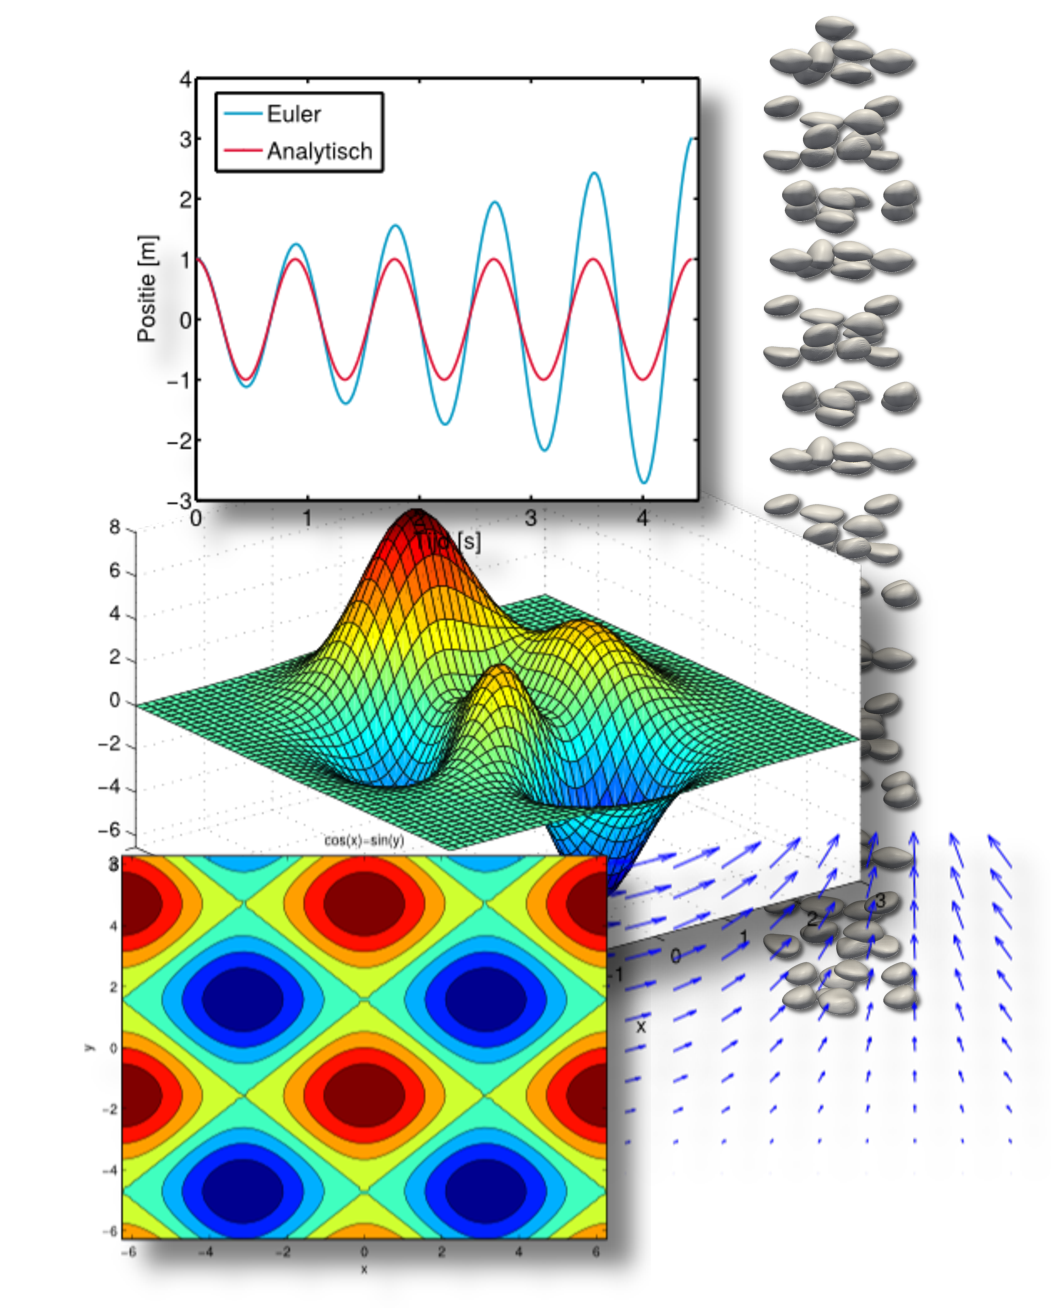
\includegraphics[width=\columnwidth]{visualisation}
 \end{columns}
\end{frame}

\begin{frame}[fragile]
  \frametitle{Plotting}
  \begin{lstlisting}
x = -5:0.1:5;
y = x.^2-4*x+3;
y2 = y + (2-4*rand(size(y))); (*@ \pause @*)
subplot(2,1,1); plot(x,y,'-',x,y2,'r.');
xlabel('X'); ylabel('Y'); title('Graph and Scatter'); (*@ \pause @*)
subplot(2,1,2); plot(x,abs(y-y2),'r-');
xlabel('X'); ylabel('Y'); title('Absolute error');
  \end{lstlisting}
  \centering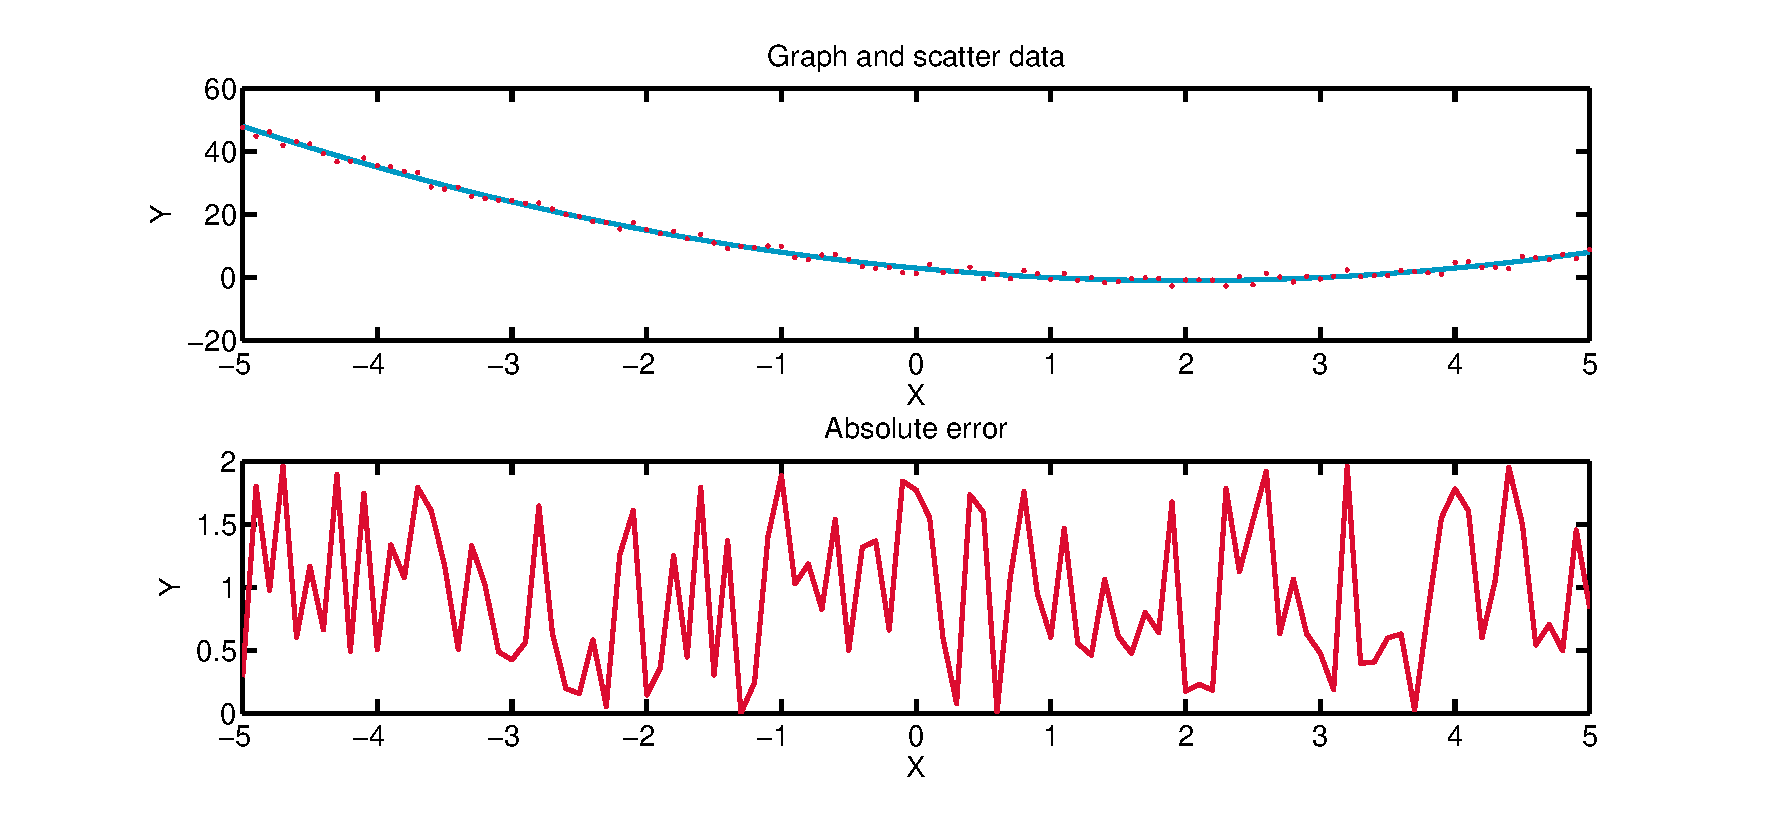
\includegraphics[width=0.8\textwidth]{showplot-utc}
\end{frame}

\begin{frame}[fragile]
  \frametitle{Animating plots}
  The \lstinline$drawnow$ command holds the execution of your program until the graph is updated. It allows to have a live view of a simulation result.
  \begin{lstlisting}
x = -5:0.1:5;
y = x.^2-4*x+3;
y2 = y + (2-4*rand(size(y)));
for i = 1:length(x)
    subplot(2,1,1); 
    plot(x(1:i),y(1:i),'-',x(1:i),y2(1:i),'r.');
    xlabel('X'); ylabel('Y'); title('Graph and Scatter');
    axis([min(x) max(x) min(y) max(y)])
    
    subplot(2,1,2); 
    plot(x(1:i),abs(y(1:i)-y2(1:i)),'r-');
    xlabel('X'); ylabel('Y'); title('Absolute error');
    axis([min(x) max(x) 0 2])

    drawnow
end
      \end{lstlisting}
\end{frame}

% \begin{frame}[fragile]
%   \frametitle{Plotting (2)}
%   Easy plotting of functions can be done using the ezplot function: \lstinline$ezplot('x-sin(x)', [0 2*pi])$:
%   \\
%   {\centering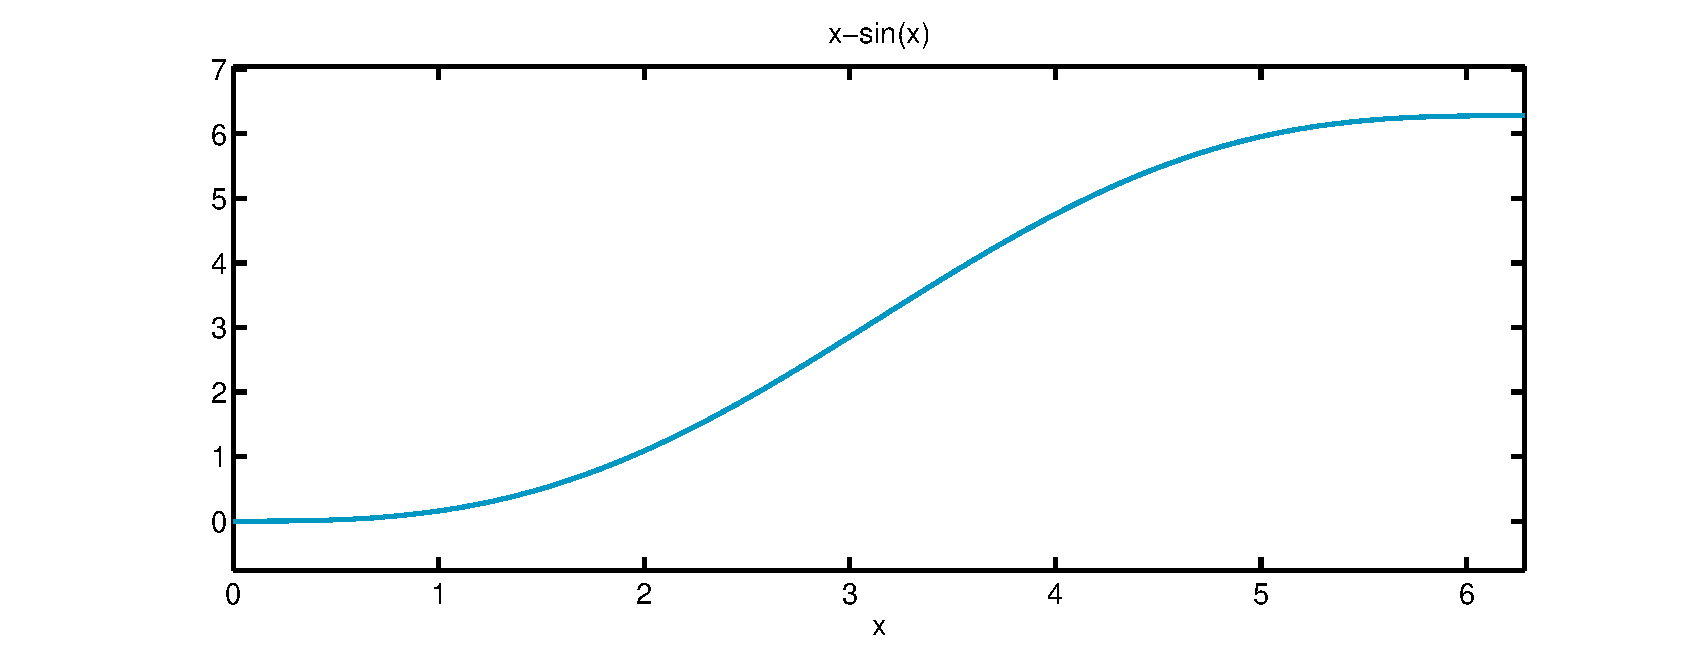
\includegraphics[width=0.5\textwidth]{show_ezplot-utc}}\\
%   Be careful with steep gradients: \lstinline$ezplot('x-sin(1/x)', [0 1])$% (use \lstinline$fplot$ instead)
%   \\
%   \centering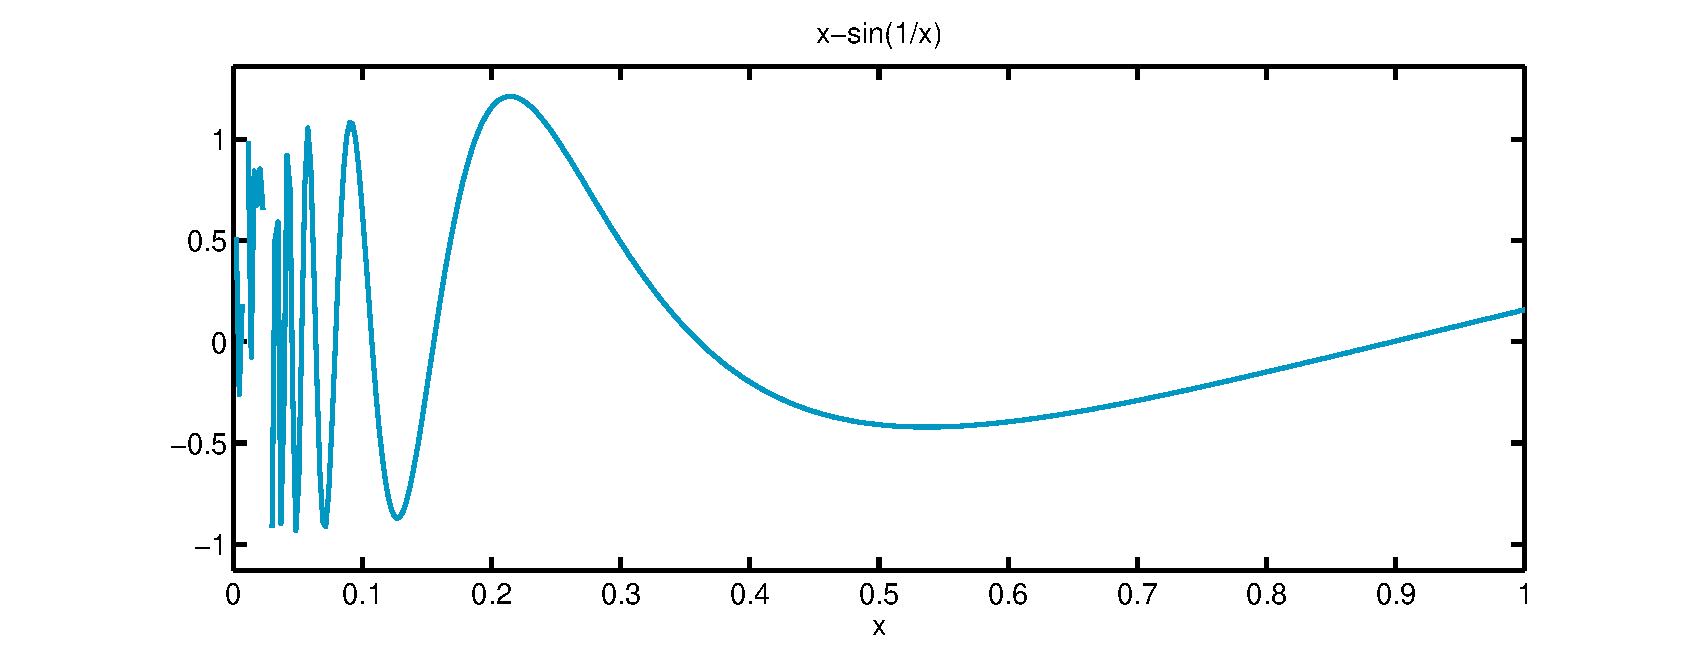
\includegraphics[width=0.5\textwidth]{show_ezplot2-utc}
% \end{frame}

\begin{frame}[fragile]
  \frametitle{Other plotting tools}
  \begin{columns}
   \column{0.6\textwidth}
    \begin{itemize}[<+->]
      \item Errorbars: \lstinline$errorbar(x,y,err)$
      \item 3D-plots: \lstinline$plot3(x,y,z)$
      \item Histograms: \lstinline$histogram(x,20)$
%       \item Vectorplots: \lstinline$quiver(x,y,vx,vy)$
    \end{itemize}
   \column{0.4\textwidth}
      \includegraphics<1>[width=\columnwidth]{show_errorbar-utc}
      \mode<presentation>{
        \includegraphics<2>[width=\columnwidth]{show_ezplot3-utc}
        \includegraphics<3>[width=\columnwidth]{show_hist-utc}
    }
%     \includegraphics<3>[width=\columnwidth]{show_quiver-utc}
 \end{columns}
\end{frame}

\subsection*{Multi-dimensional data}
\begin{frame}<handout:3>[fragile]
  \frametitle{Multi-dimensional data}
  Matlab typically requires the definition of rectangular grid coordinates using \lstinline$meshgrid$:\\
  \begin{overlayarea}{\textwidth}{6cm}
  \begin{columns}[T]
   \column{0.6\textwidth}
    \begin{lstlisting}
[x y] = meshgrid(-2:0.1:2, -2:0.1:2);
z = x .* y .* exp(-x.^2 - y.^2);
    \end{lstlisting}
    \vskip1em
    \begin{itemize}
      \item<2-> Surface plot
      \item<3-> Contour plot
      \item<4-> Waterfall 
      \item<5> Ribbons
    \end{itemize}
   \column{0.4\textwidth}
   \begin{center}
      \includegraphics<2>[width=\columnwidth]{show_surf}
      \mode<presentation>{
        \includegraphics<3>[width=\columnwidth]{show_contour}
        \includegraphics<4>[width=\columnwidth]{show_waterfall}
        \includegraphics<5>[width=\columnwidth]{show_ribbon}
      }
   \end{center}
    \only<2>{
      \lstinline$surf(x,y,z);$
    }
    \mode<presentation>{
      \only<3>{
        \lstinline$v=-0.5:0.05:0.5;$ \\
        \lstinline$contour(x,y,z,v,'ShowText', 'on');$
      }
      \only<4>{
      \lstinline$waterfall(x,y,z);$\\
      \lstinline$colormap(winter);$
      }
      \only<5>{
      \lstinline$ribbon(z);$
      }
    }
 \end{columns}
 \end{overlayarea}
\end{frame}

\begin{frame}[fragile]
  \frametitle{Vector data}
  The gradient operator, as expected, is used to obtain the gradient of a scalar field. Colors can be used in the background to simultaneously plot field data:
  \begin{columns}[T]
   \column{0.6\textwidth}
    \begin{lstlisting}
[x y] = meshgrid(-2:0.2:2, -2:0.2:2);
z = x .* y .* exp(-x.^2 - y.^2)
[dx dy] = gradient(z,8,8)

% Background
contourf(x,y,z,30,'LineColor','none');
colormap(hot); colorbar;

axis tight; hold on;

% Vectors
quiver(x,y,dx,dy,'k');
    \end{lstlisting}
   \column{0.4\textwidth}
   \begin{center}
      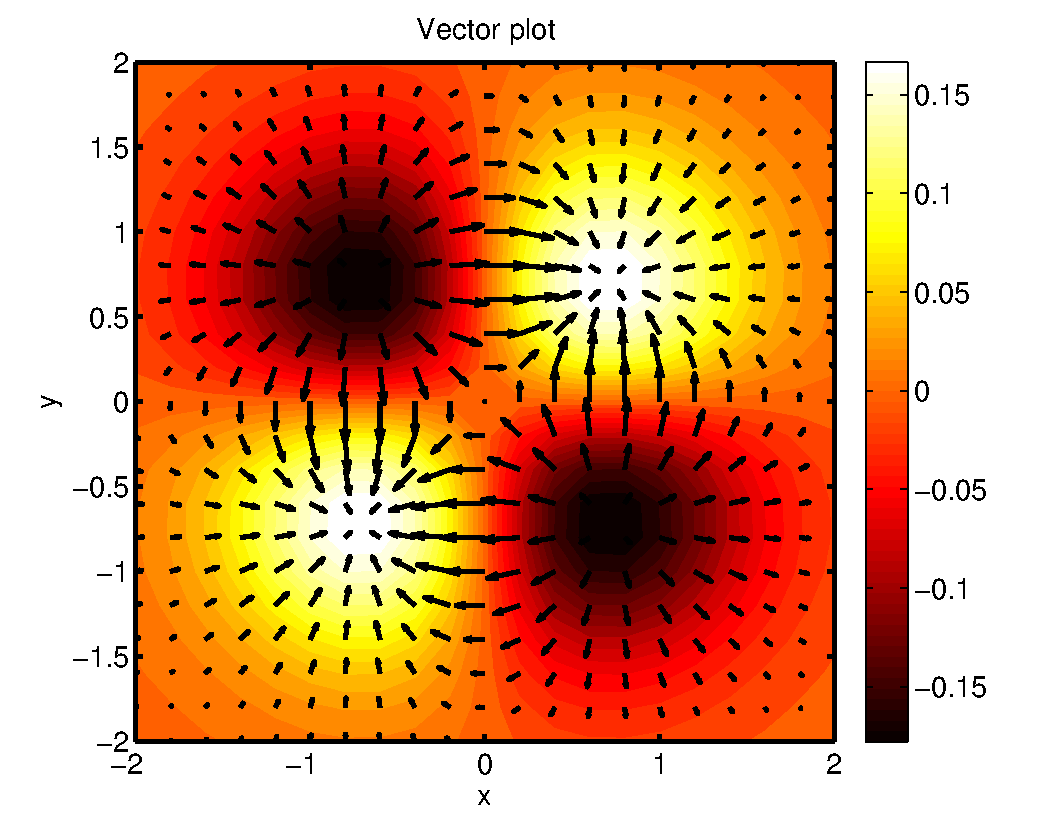
\includegraphics[width=\columnwidth]{show_vector}
    \end{center}
  \end{columns}
\end{frame}

\section{Functions: revisited}
\againframe<2>{contents_prog2}
\subsection*{Function handles}
\begin{frame}[fragile]
  \frametitle{Functions: revisited}
  In MATLAB you can define your own functions to re-use certain functionalities. We now define the mathematical function $f = x^2+e^x$:
  \begin{lstlisting}
function y = f(x)
y = x.^2 + exp(x);
  \end{lstlisting}
  \pause
  Note:
  \begin{itemize}
    \item The first line of the file has to contain the \lstinline$function$ keyword
    \item The variables used are \emph{local}. They will not be available in your Workspace
    \item The file needs to be saved with the same name as the function, i.e. ``f.m''
    \item The semi-colon prevents that at each function evaluation output appears on the screen
    \item If \lstinline$x$ is an array, then \lstinline$y$ becomes an array of function values.
  \end{itemize}
\end{frame}

\begin{frame}[fragile]
  \frametitle{Anonymous functions}
  If you do not want to create a file, you can create an \emph{anonymous function}:
  \begin{lstlisting}
>> f = @(x) (x.^2+exp(x))
  \end{lstlisting}
  \pause
  \begin{itemize}
    \item \lstinline$f$: the name of the function
    \item \lstinline$@$: the function handle
    \item \lstinline$x$: the input argument
    \item \lstinline$x.^2+exp(x)$: the actual function
  \end{itemize}\pause
  \begin{lstlisting}
>> f(0:0.1:1)   
  \end{lstlisting}
\end{frame}

\begin{frame}[fragile]
  \frametitle{Using function handles}
  A function handle points to a function. It behaves as a variable
  \begin{lstlisting}
>> myFunctionHandle = @exp 
>> myFunctionHandle(1)
  \end{lstlisting}
  \pause
  Used a.o. for passing a function to another function, for instance for optimization functions.
  \[ f(x) = x^3 -x^2 -3\arctan{x}+1 \]
  \pause
  Matlab offers a function \lstinline$fzero$ that can find the roots of a function in a certain range:
  \begin{lstlisting}
>> f = @(x) x.^3 - x.^2 - 3*atan(x) + 1;
>> fzero(f,[-2 2])
>> ezplot(f)
>> f(ans)
  \end{lstlisting}
\end{frame}

\begin{frame}[fragile]
  \frametitle{Practice function handles}
  Consider the function
  \[ f(x) = -x^2 - 3x + 3 + e^{x^2} \]
  The built-in Matlab function \lstinline$fminbnd$ allows to find the minimum of a function in a certain range. Find the minimum of $f(x)$ on $-2\leq x \leq2$.
  Example usage:
  \begin{lstlisting}
x = fminbnd(fun,x1,x2)
  \end{lstlisting}
  \pause
  Answer using an anonymous function:
  \begin{lstlisting}
>> f = @(x) -x.^2 - 3*x + 3 + exp(x.^2)
>> ezplot(f,[-2 2])
>> fminbnd(f,-2,2)
>> f(ans)
  \end{lstlisting}
  \pause
  Various related functions are \lstinline$fzero$, \lstinline$feval$, \lstinline$fsolve$, \lstinline$fminsearch$. They will be discussed later in the course.
\end{frame}

\section{Concluding remarks}
\subsection*{Advanced}
\againframe<2>{contents_prog2}
\begin{frame}
  \frametitle{Advanced concepts}
  \begin{itemize}
    \item Object oriented programming: classes and objects
    \item Memory management: some programming languages require you to allocate computer memory yourself (e.g. for arrays)
    \item External libraries: in many cases, someone already built the general functionality you are looking for
    \item Compiling and scripting (``interpreted''); compiling means converting a program to computer-language before execution. Interpreted languages do this on the fly.
    \item Parallellization: Distributing expensive calculations over multiple processors or GPUs.
  \end{itemize}\pause
     \only<beamer>{
       \tikzstyle{every picture}-=[remember picture]
       \begin{tikzpicture}[remember picture,overlay]{
   \node at (current page.center) {
\includegraphics[width=\textwidth]{fullnerd2.png}};}
       \end{tikzpicture}}
 \end{frame}

\againframe{workrightfast}
\againframe{wrf-explain}

\subsection*{Exercise}
\begin{frame}<handout:1-2>
  \frametitle{Exercise: finding the roots of a parabola}
  We are writing a program that finds for us the roots of a parabola. We use the form
  \[
    y = ax^2 + bx + c
  \]
  \pause
  What is our program in pseudo-code? \pause
  \begin{enumerate}[<+->]
    \item Input data ($a$, $b$ and $c$)
    \item Identify special cases ($a=b=c=0$, $a=0$)
    \begin{description}
      \item[$a=b=c=0$] Solution indeterminate
      \item[$a=0$] Solution: $x = -\frac{c}{b}$
    \end{description}
    \item Find $D = b^2-4ac$
    \item Decide, based on $D$:
    \begin{description}
      \item[$D<0$] Display message: complex roots
      \item[$D=0$] Display 1 root value
      \item[$D>0$] Display 2 root values
    \end{description}
  \end{enumerate}
\end{frame}

\begin{frame}<handout:0>[plain,fragile]
  \frametitle{Example: finding the roots of a parabola}
  \small\selectfont
  \begin{lstlisting}[basicstyle=\scriptsize\ttfamily]
function x = parabola(a,b,c)
% Catch exception cases
if (a==0)
    if(b==0)
        if(c==0)
            disp('Solution indeterminate'); return;
        end
        disp('There is no solution');
    end
    x = -c/b;
end

% Compute determinant
D = b^2 - 4*a*c;
if (D<0)
    disp('Complex roots'); return;
    else if (D==0)
        x = -b/(2*a);
        else if (D>0)
                x(1) = (-b + sqrt(D))/(2*a);
                x(2) = (-b - sqrt(D))/(2*a);
                x = sort(x);
        end
    end
end
  \end{lstlisting}
\end{frame}

\begin{frame}[fragile]
  \frametitle{Example: finding the roots of a parabola}
  \begin{lstlisting}
>> roots([1 -4 -3])
ans =
    4.6458
   -0.6458
  \end{lstlisting}
\end{frame}



%
%\subsection*{Projectile}
%\begin{frame}[fragile]
%\scriptsize\selectfont
%  \frametitle{Example: projectile trajectory}
%  \begin{center}
%    \begin{tikzpicture}[scale=0.7,ball/.style={circle,minimum size=8mm,thick,shading=ball,ball color=maincolor,
%				      font=\sffamily\scriptsize},>=stealth',thick,node distance=0.75cm]
%      \node[ball,anchor=north] (ball) at (0,0) {$M$};
%      \node[anchor=north east] at (1.5,1.7) (aim) {};
%      \node[anchor=south east] at (aim.south) {$v_0$};
%      \uncover<2->{\node at (7.5,-0.5) (aim2) {};
%      \node[anchor=north] at (aim2) {Trajectory};}    
%      \node at (4,2.6) (aim3) {};
%      \uncover<3->{\node[ball,ball color=gray,fill opacity=0.5] (ball2) at (aim3) {};}
%      
%      \draw[->] (ball.north east) -> (aim.center);
%      \draw<2->[->,dashed] (ball.north east) parabola bend (aim3) (aim2);
%      \draw<3->[->] (ball2) -- node[midway,anchor=west]{$F_g=mg$} ($ (ball2)+(0,-2) $);
%    \end{tikzpicture}
%  \end{center}
%  \vskip1em
%  \begin{itemize}
%    \item<1-> A ball with mass $M$ is thrown at time $t = 0$ with a certain velocity $v(t) = v(0) = v_0$
%    \item<2-> We need to describe the trajectory of the ball over time
%    \item<3-> It is given that the only force acting on the ball is gravity: $F = Mg$
%  \end{itemize}
%\end{frame}
%
%\begin{frame}[fragile]
%\scriptsize\selectfont
%  \frametitle{Example: projectile trajectory}
%  Computers cannot solve a continuous equation; we need to \emph{discretize} the time into steps of size $\Delta t$. Create a time line:\\ \vskip2em\pause
%  \begin{tikzpicture}[snake=zigzag, line before snake = 5mm, line after snake = 5mm]
%    %draw horizontal line   
%    \draw (0,0) -- (6,0);
%    \draw[snake] (5.5,0) -- (8.5,0);
%    \draw (8,0) -- (10,0);
%
%    %draw vertical lines
%    \foreach \x in {0,2,4,6,8,10}
%      \draw (\x cm,3pt) -- (\x cm,-3pt);
%
%    %draw nodes
%    \draw (0,0) node[below=3pt] {$ t=0 $} node[above=3pt] {$ 1 $};
%    \draw (2,0) node[below=3pt] {$ \Delta t $} node[above=3pt] {$ 2 $};
%    \draw (4,0) node[below=3pt] {$ 2\Delta t $} node[above=3pt] {$ 3 $};
%    \draw (6,0) node[below=3pt] {$ 3\Delta t $} node[above=3pt] {$ 4 $};
%    \draw (8,0) node[below=3pt] {$ t_\mathrm{end}-\Delta t $} node[above=3pt] {$ n-1 $};
%    \draw (10,0) node[below=3pt] {$ t_\mathrm{end} $} node[above=3pt] {$ n $};
%    
%    \onslide<4>{
%      \draw (0,-1.5) node[above=1pt] {$x_0$};
%      \draw (0,-1.5) node[below=3pt] {$v_0$};
%    }
%    \onslide<5>{
%      \draw (0,-1.5) node[above=1pt] {$x(t)$};
%      \draw (0,-1.5) node[below=3pt] {$v(t)$};
%      \draw (2,-1.5) node[above=1pt] {$x(t+\Delta t)$};
%      \draw (2,-1.5) node[below=3pt] {$v(t+\Delta t)$};
%    }
%    \onslide<6>{
%      \draw (2,-1.5) node[above=1pt] {$x(t)$};
%      \draw (2,-1.5) node[below=3pt] {$v(t)$};
%      \draw (4,-1.5) node[above=1pt] {$x(t+\Delta t)$};
%      \draw (4,-1.5) node[below=3pt] {$v(t+\Delta t)$};
%    }
%    \onslide<7>{
%      \draw (4,-1.5) node[above=1pt] {$x(t)$};
%      \draw (4,-1.5) node[below=3pt] {$v(t)$};
%      \draw (6,-1.5) node[above=1pt] {$x(t+\Delta t)$};
%      \draw (6,-1.5) node[below=3pt] {$v(t+\Delta t)$};
%    }
%   \end{tikzpicture}
%\end{frame}
%
%\begin{frame}[fragile]
%\scriptsize\selectfont
%  \frametitle{Example: projectile trajectory}
%  \begin{itemize}
%    \item A Taylor expansion shows how the $x$-position is obtained at discrete time intervals: 
%    \[ f(x) = f(a) + \frac{f'(a)}{1!}(x-a) + \frac{f''(a)}{2!}(x-a)^2  + \ldots \]\pause
%    \[ x(t+\Delta t) = x(t) + \frac{\frac{dx}{dt}(t)}{1!}(t + \Delta t - t) + \frac{\frac{d^2x}{dt^2}}{2!}(t+\Delta t - t)^2  + O(\Delta t^3) \] \pause
%    \[ x(t+\Delta t) = x(t) + v(t)\Delta t + \frac{F}{2M}\Delta t^2  + O(\Delta t^3) \] \pause
%    \item Taking small time steps, we can discard $\Delta t^2$ and subsequent terms:
%    \[ x(t+\Delta t) = x(t) + v(t)\Delta t \] \pause
%    \item A similar approach is taken for the velocity:
%    \[ v(t+\Delta t) = v(t) + a(t)\Delta t \] \pause
%    \[ F = Ma \Rightarrow a = \frac{F}{M} \Rightarrow v(t+\Delta t) = v(t) + \frac{F(t)}{M}\Delta t \]
%  \end{itemize}
%\end{frame}
%
%\begin{frame}[fragile]
%\scriptsize\selectfont
%  \frametitle{Example: projectile trajectory}
%  Our mathematical model is as follows: \pause
%  \begin{enumerate}
%    \item Initialisation of parameters ($x_0$, $v_0$, $g$, $\Delta t$, $t_end$, $M$)\pause
%    \item Create storage vectors for time, position, velocity \pause
%    \item Start a time-marching loop \pause
%    \begin{itemize}
%    \scriptsize\selectfont
%      \item Calculate $x(t+\Delta t)$, then $F$, then $v(t+\Delta t)$:
%      \[ x(t+\Delta t) = x(t) + v(t)\Delta t \] 
%      \[ F = Mg \]
%      \[ v(t+\Delta t) = v(t) + \frac{F}{M}\Delta t \] \pause
%      \item Store current solution
%    \end{itemize}
%    \item Draw result and return solution vector $x$
%    \begin{itemize}
%      \item Exact solution:
%      \[
%        x(t) = x_0 + v_0 t + ( \frac{1}{2} -9.81 t^2 )
%      \]
%    \end{itemize}
%  \end{enumerate}
%\end{frame}
%
%\begin{frame}[fragile]
%  \frametitle{Example: projectile trajectory - solution (initialisation)}
%  \scriptsize\selectfont
%  \begin{lstlisting}
%function [pos,tim] = projectile(v0,M)
%
%% Initialise parameters
%t_end = 2;                  % End time
%deltat = 0.01;              % Time step
%x0 = 1;                     % Initial position
%
%nsteps = fix(t_end/deltat); % Number of time steps
%pos = zeros(nsteps,1);      % Position vector
%vel = zeros(nsteps,1);      % Velocity vector
%tim = zeros(nsteps,1);      % Time vector
%
%% Default values for mass and velocity
%if (nargin < 2)
%    M = 10;
%    if (nargin < 1)
%        v0 = 1;
%    end
%end
%  \end{lstlisting}
%\end{frame}
%
%\begin{frame}[fragile]
%  \frametitle{Example: projectile trajectory - solution (main program)}
%  \scriptsize\selectfont
%  \begin{lstlisting}
%pos(1) = x0;                % Store initial position
%vel(1) = v0;                % Store initial velocity
%
%% The time loop
%for n = 1:nsteps-1
%    pos(n+1) = position(pos(n),vel(n),deltat);
%    vel(n+1) = velocity(vel(n),M,deltat);
%    tim(n+1) = tim(n) + deltat;
%end
%
%% Plot results
%figure; plot(tim,pos, 'o');
%
%% Compare to analytical solution
%compareToExact(x0,v0,tim,pos);
%
%end
%  \end{lstlisting}
%\end{frame}
%
%\begin{frame}[fragile]
%  \frametitle{Example: projectile trajectory - solution (added functions)}
%  \scriptsize\selectfont
%  \begin{lstlisting}
%function F = force(M)
%% M:    mass of particle
%g = -9.81;
%F = M * g;
%end
%
%function v = velocity(vt,mass,dt)
%% vt:   velocity at previous time
%% mass: mass of particle
%% dt:   time step size
%v = vt + force(mass)/mass * dt;
%end
%
%function x = position(xt,vel,dt)
%% xt:   position at current time step
%% vel:  velocity at current time step
%% dt:   time step size
%x = xt + vel * dt;
%end
%  \end{lstlisting}
%\end{frame}
%
%\begin{frame}[fragile]
%  \frametitle{Example: projectile trajectory - solution (verification)}
%  \scriptsize\selectfont
%  \begin{lstlisting}
%function compareToExact(x0,v0,tim,pos)
%
%% Exact solution
%pos_ex = x0 + v0 * tim + ( 0.5 * -9.81 * tim .* tim );
%
%% Draw comparative figure
%figure;
%subplot(2,1,1)
%plot(tim,pos, 'o');
%hold on;
%plot(tim,pos_ex,'r-')
%subplot(2,1,2)
%stem(tim,pos_ex-pos,'r-')
%
%% Print the L2-error norm
%norm(pos_ex - pos)
%end
%  \end{lstlisting}
%\end{frame}
%
%\begin{frame}
%  \frametitle{Example: projectile trajectory - solution}
%  \begin{center}
%    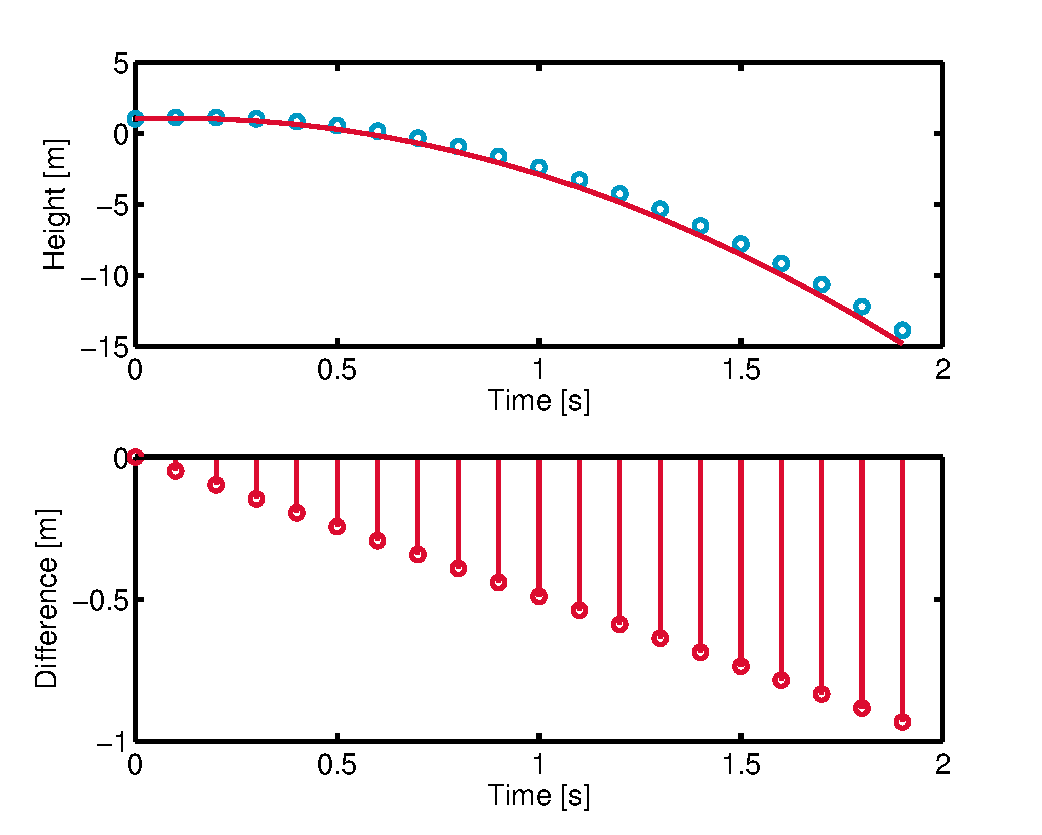
\includegraphics[width=0.8\textwidth]{projectile-utc}
%  \end{center}
%\end{frame}